
\section*{Contemplación y EDGES} % Espacio para hablar del proyecto de (acomplete) de Dorian

\iffalse
\begin{itemize}
\item Distopía
\item domo 
\item Underborders
\item Milena y Concepción
\item setInterval()
\item Contemplación del fin del Mundo
\item sistemas mixtos
\item espacio y performance fusionados en Contemplación
\end{itemize}
\fi

\color{BlueViolet}

Una de las reflexiones que estuvo presente desde el inicio del proyecto partió de las distinciones más inmediatas: mundos virtuales / mundos reales, materialidad / inmaterialidad. Consideramos que procesos como los de \textit{Panorama} transitan entre la extensión de la fisicalidad hacia la virtualidad\footnote{`la trascendencia de la fisicalidad del mundo virtual nos permite extender nuestro modo de operación en el mundo físico. Nuevas formas de viaje, una nueva forma de comunicación, una nueva forma de operación, un nuevo medio de expresión" pp. 49} \citep{cyberspace} y la reconfiguración de la materialidad\footnote{``el arte no solamente podría ser performeado en el plano sensorial, sino también en el plano inteligible. Las estéticas de la participación y la constitución de los medios digitales podrían intepretarse como la continuación de algunos de esos prinicipios." pp 190} \citep{andreasosa} de cara al giro digital que posibilita la continuación y contraposición estéticas y formas de organización social. 

\color{black}

\textit{Distopía}, \textit{NLXS + NK}, \textit{Interconexión}, \textit{setInterval()} y \textit{La Contemplación del Fin del Mundo} fueron los eventos realiados en el marco de \textit{EDGES}. 

\begin{figure}[H]
  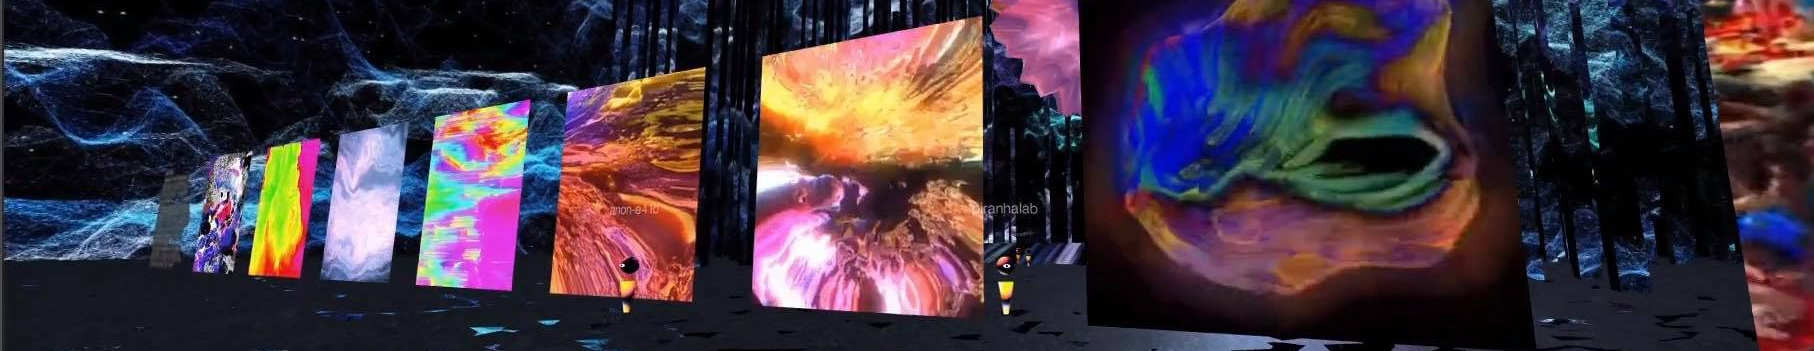
\includegraphics[width=\textwidth]{img/distopia.png}
  \caption{EDGES Distopía. Imágenes: LVSTVCRV}
\end{figure}

\textit{La Contemplación del Fin del Mundo} es un performance a modo de ejuego, último evento de la serie \textit{EDGES} que destruye el escenario de manera simbólica para dar por finalizado el ciclo de conciertos. Los asistentes podían presenciar el fin del mundo con la destrucción del escenario y otros eventos como inundaciones, objetos celestiales y finalmente la dispersión de los colores del escenario, dejando a los objetos del espacio sin razgos reconocibles.

La idea principal sirvió como vehículo para la exploración del espacio como característica del performance, el mundo explorable, la persecución en forma de figuras celestiales que ocupaban todo el espacio o que se expandían e iluminaban todo así como las inundaciociones. También permitió la exploración del uso de pantallas distribuidas a lo largo de todo el mundo, permitiendo a los usuarios presenciar el performance desde cualquier ubicación.

Uno de los aspectos a destacar de este concierto es el uso de acciones colectivas lanzadas por el artista, que durante el trascurso del evento podía cambiar las características del ambiente de manera similar entre los participantes. La experiencia de los usuarios fue se transformaba en el trancurso del evento, fue homogénea y compartida. Adicionalmente se implementó Hydra \citep{hydra} como un framework externo para la creación de visuales.

Las dificultad de las experiencias compartidas radica en la sincronización de eventos, tanto para los usuarios que ingresan desde el inicio o los usuarios ocasionales, sin importar ubicación geográfica o dispositivo. Esta posibilidad permite la interacción del artista y genera situaciones que añadan dinámica al juego, donde los asistentes se desplazan de ser observadores a ser participantes activos.

% Escribir sobre el proyecto de vincular threejs y hydra 

\color{Fuchsia}

Manifiestos, posturas políticas y alternativas en la organización que dialogan con la escritura de software como desarrollo tecnológico y como acto creativo. Por ejemplo \textit{live coding} y la transparencia de los procesos o el uso de interfaces de texto \citep{collinsLivecoding}, el manifiesto de una servidora feminista \citep{feministserver} o la arquitectura de distribución de información par a par\footnote{\textit{P2P} (par a par) por sus siglas en inglés.  ``La arquitectura de una red distribuida puede ser llamada Par a Par (P-to-P, P2P, ...)   si los participantes comparten una parte de los recursos de su propio software (poder de procesamiento, capacidad de almacenamiento, capacidad de conexión a la red, impresoras,...) Estos recursos compartidos son necesarios para proveer el Servicio y el contenido ofrecido por la red... Estos son accedidos por otros pares directamente sin pasar por entidades intermediarias." \citep{p2p}} que persigue la distribución y la descentralización en redes que posibilitan espacios virtuales \citep{cyberspace} y que incluso puede extenderse al autocuidado y formas alternativas de expresar relaciones sociales en red \citep{dwc}. 

\color{black}
